\documentclass[handout]{beamer}

\usepackage{Haust2017glærur}

\title{Stærðfræðimynstur í tölvunarfræði}
\subtitle{Vika 5, fyrri fyrirlestur}

\begin{document}

\begin{frame}
\titlepage
\end{frame}


\section{Inngangur}

\begin{frame}{Í síðasta tíma}
\begin{itemize}
 \item Reikniflækja
 \item Tímaflækjur nokkurra reiknirita
 \item Mengin $P$ og $NP$
\end{itemize}
\end{frame}

\section{Talnafræði}

\begin{frame}{Talnafræði}
\begin{itemize}
 \item Stærðfræði heiltalna kallast talnafræði
 \item Löng og mikil saga
 \begin{itemize}
  \item Fræg forn-grísk nöfn sem koma við sögu: Evklíð, Eratosþenes
 \end{itemize}
 \item Stærðfræði prímtalna fellur undir talnafræði
\end{itemize}
\end{frame}

\section{Deiling og afgangur}

\begin{frame}{Deilanleiki}
Ýmis hugtök í talnafræði krefjast skilnings á deilanleika (e. \emph{divisibility})

\begin{tcolorbox}[title=Deilanleiki]
Séu $a$ og $b$ heiltölur, $a \neq 0$, segjum við að $a$ deili (e. \emph{divides}) $b$ ef til er heiltala $c$ svo að $b = ac$, þ.e.a.s. ef $\frac{b}{a}$ er heiltala.

Þegar $a$ deilir $b$ segjum við að $a$ sé deilir (e. \emph{divisor} eða \emph{factor}) $b$ og að $b$ sé margfeldi (e. \emph{multiple}) af $a$.

Við skrifum $a \mid b$ þegar $a$ deilir $b$, annars $a \nmid b$.
\end{tcolorbox}
\end{frame}

\begin{frame}{Deilanleiki - dæmi}
Er $3\mid 7$? \pause

Nei, $7/3$ er ekki heiltala. \pause

\vspace{0.5cm}
Er $3\mid 12$? \pause

Já, $12/3$ er heiltalan $4$.
\end{frame}

\begin{frame}{Eiginleikar deilanleika}
Heiltöludeiling hefur nokkra áhugaverða eiginleika
\begin{tcolorbox}[title=Eiginleikar deilanleika]
Séu $a$, $b$ og $c$ heiltölur, $a \neq 0$, þá gildir:
\begin{enumerate}
 \item Sé $a\mid b$ og $a\mid c$, þá $a\mid (b+c)$
 \item Sé $a\mid b$, þá $a\mid b\cdot c$
 \item Sé $a\mid b$ og $b\mid c$, þá $a\mid c$
\end{enumerate}
\end{tcolorbox}
\end{frame}

\begin{frame}{Deilingarreikniritið}
Deilingarreikniritið (e. \emph{the division algorithm}) er ekki reiknirit, heldur setning.

\begin{tcolorbox}[title=Deilingarreikniritið]
Látum $a$ og $d$ vera heiltölur, $d > 0$. 
Þá eru til heiltölur $q$ og $r$, $0 \leq r < d$ svo að $a = dq +r$.
\end{tcolorbox}

Hér er $d$ deilir, $a$ deilistofn (e. \emph{dividend}), $q$ kvóti (e. \emph{quotient}) og $r$ afgangur (e. \emph{remainder}).
\end{frame}


\begin{frame}{Kvóti og afgangur}
Um deilinn $d$, deilistofninn $a$, kvótann $q$ og afganginn $r$ má rita:
\[
 q = a \text{ div } d
\]
og
\[
 r = a \text{ mod } d
\]
Athugum að div og mod eru föll.
\end{frame}

\begin{frame}{Dæmi um deilingu}
Hverjir eru kvótinn og afgangurinn þegar deilistofninn er $101$ og deilirinn $11$?\pause

Höfum
\[
 101 = 11 \cdot 9 + 2
\]

Svo kvótinn er $101 \text{ div } 11 = 9$ og afgangurinn $101 \Mod 11 = 2$.

\end{frame}

\begin{frame}{Dæmi um deilingu}
Hverjir eru kvótinn og afgangurinn þegar deilistofninn er $-11$ og deilirinn $3$?\pause

Höfum
\[
 -11 = 3 \cdot (-4) + 1
\]

Svo kvótinn er $-11 \text{ div } 3 = -4$ og afgangurinn $-11 \Mod 3 = 1$.

\vspace{0.5cm}
Athugum að þó að $-11 = 3(-3) - 2$ sé satt, þá uppfyllir jafnan ekki $0 \leq r < 3$.
\end{frame}

\begin{frame}{Varúð - forritunarmál}
\begin{itemize}
 \item Forritunarmál meðhöndla deilingarafgang á ýmsa vegu
 \begin{itemize}
  \item Stundum virki (\%)
  \item Stundum föll (\texttt{mod} eða \texttt{rem})
  \item Stundum meira en eitt fall\ldots
 \end{itemize}
 \item Neikvæðar tölur sérstaklega varhugaverðar
 \begin{itemize}
  \item Stundum er deilingarafganginum leyft að vera neikvæður
  \item Stundum er $a \Mod m$ skilgreint jafnvel þó að $m$ sé neikvætt eða 0
 \end{itemize}
\end{itemize}
\end{frame}

\section{Framsetning heiltalna}

\begin{frame}{Framsetning heiltalna}
\begin{itemize}
 \item Fólk í flestum menningarheimum notar tugakerfið til að setja fram tölur
 \begin{itemize}
  \item Líklega vegna þess að við höfum 10 fingur
  \item Hafa eiginleika sem byggjast á tölunni 10: $965 = 9\cdot10^2+6\cdot10^1+5\cdot10^0$
 \end{itemize}
 \item Tölvuútreikningar byggjast oftast á grunntölunni 2 (tvíundarkerfi)
 \begin{itemize}
  \item Einnig til áttundakerfi (e. \emph{octal}) með grunntöluna 8 og sextándakerfi (e. \emph{hexadecimal}) með grunntöluna 16
  \item Áttunda- og sextándakerfistölur eru oftast notaðar til að setja tvíundarkerfistölur fram fyrir fólk
 \end{itemize}
\end{itemize}
\end{frame}

\begin{frame}{Framsetning heiltalna}
Um framsetningu heiltalna gildir:

\begin{tcolorbox}[title=Framsetning heiltalna]
Látum $b$ vera heiltölu, $b > 1$. Þá getum við sett fram jákvæðu heiltöluna $n$ á sniðinu
\[
 n = a_kb^k + a_{k-1}b^{k-1} + \ldots + a_1b + a_0
\]
þar sem $k$ er ekki-neikvæð heiltala, $a_0, a_1, \ldots, a_k$ eru ekki-neikvæðar heiltölur minni en $b$ og $a_k \neq 0$.
\end{tcolorbox}
Talað er um framsetningu með grunntölunni $b$.
\end{frame}

\begin{frame}{Reiknirit til grunntöluskipta}
Gráðugt reiknirit má nota til að skipta um grunntölu:
\begin{center}
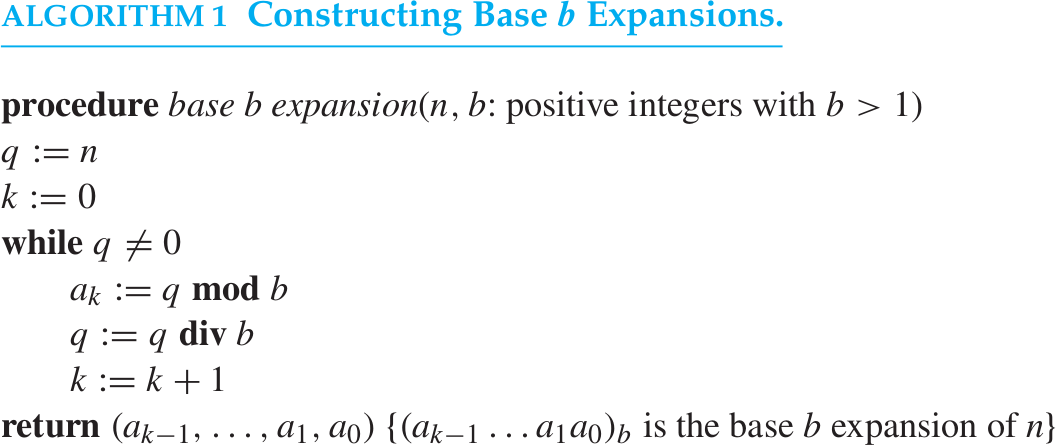
\includegraphics[width=\textwidth]{base-conversion-algorithm}
\end{center}
\end{frame}

\begin{frame}{Grunntöluskipti - dæmi}
\vspace{0.5cm}
Setjum tugakerfistöluna $(241)_{10}$ fram sem tvíundakerfistölu.
\begin{align*}
241 &= 2 \cdot 120 + 1\\
120 &= 2 \cdot 60 + 0\\
60 &= 2 \cdot 30 + 0\\
30 &= 2 \cdot 15 + 0\\
15 &= 2 \cdot 7 + 1\\
3 &= 2 \cdot 1 + 1\\
1&= 2 \cdot 0 + 1\\
\end{align*}

\vspace{-0.8cm}
Fáum afgangana $1, 0, 0, 0, 1, 1, 1, 1$ svo
\[
 (241)_{10} = (11110001)_2
\]
\end{frame}

\begin{frame}{Grunntölurnar 2, 8 og 16}
    Mjög einfalt er að breyta á milli grunntalnanna 2, 8 og 16 beint.
    \vspace{0.5cm}

    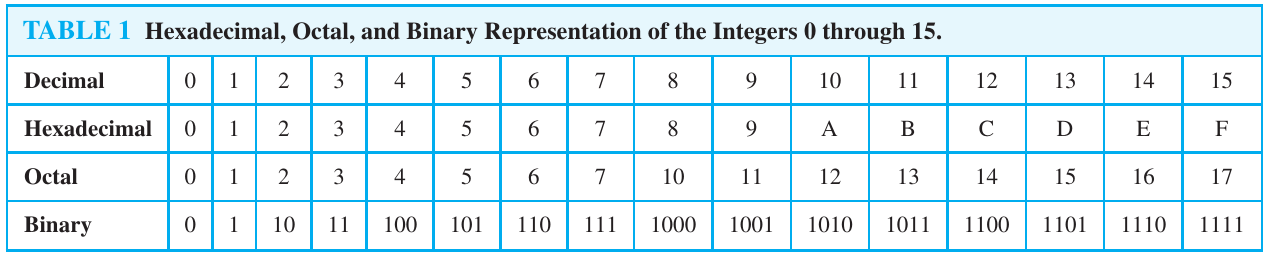
\includegraphics[width=\textwidth]{binary-equiv}

    Dæmi: $(765)_8$ inniheldur blokkirnar $111$, $110$ og $101$.\\
    \[
        (765)_8 = (111 110 101)_2
    \]
\end{frame}

\begin{frame}{Samlagning tvíundartalna}
Hægt er að skilgreina reiknirit til samlagningar á tvíundartölum
\begin{center}
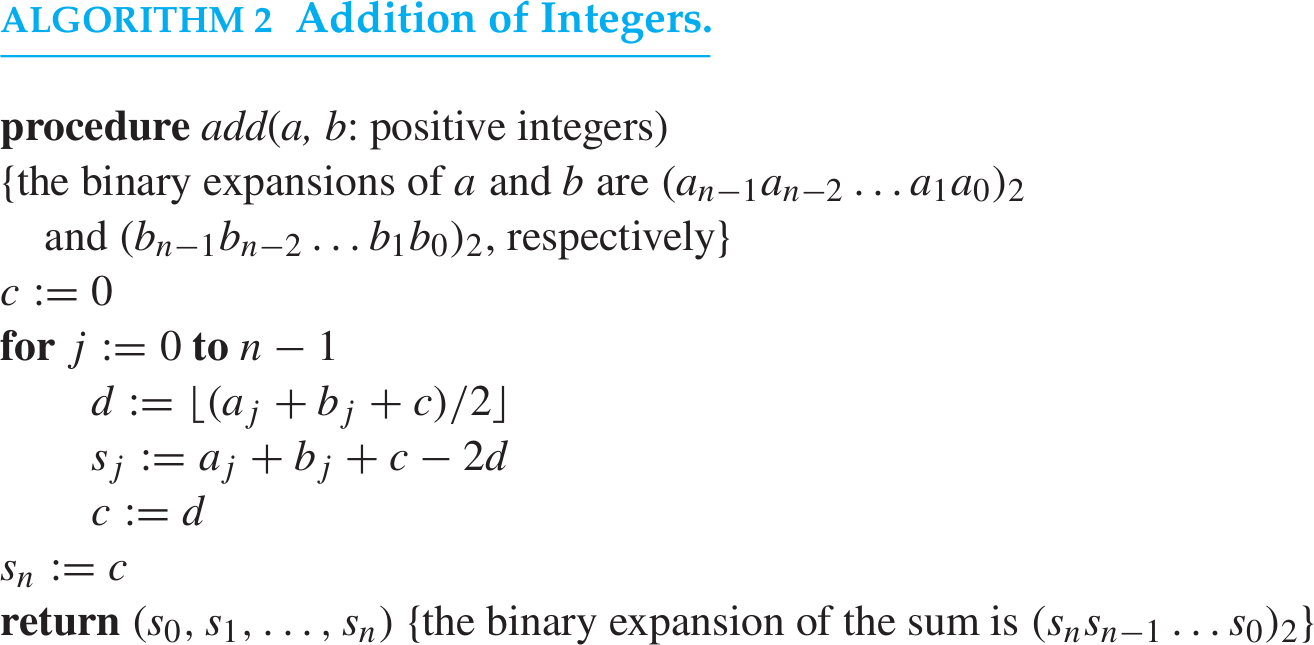
\includegraphics[width=0.9\textwidth]{binary-addition}
\end{center}
\end{frame}

\section{Prímtölur}

\begin{frame}{Prímtölur}
\begin{tcolorbox}[title=Prímtölur]
Heiltala $p$ stærri en 1 er prímtala (e. \emph{prime}) ef einu deilar $p$ eru 1 og $p$ sjálft. Heiltala stærri en 1 sem ekki er prímtala er samsett tala (e. \emph{composite}).
\end{tcolorbox}
\end{frame}

\begin{frame}{Grundvallarsetning}
``The fundamental theorem of arithmetic'' er eftirfarandi:

\begin{tcolorbox}[title=Fundamental theorem of arithmetic]
Hver heiltala stærri en 1 er prímtala eða margfeldi tveggja eða fleiri prímtalna sem skrifa má í stígandi röð.
\end{tcolorbox}

Það að finna prímtölurnar sem mynda samsetta tölu þegar þær eru margfaldaðar saman kallast að finna prímtöluþætti samsettu tölunnar.
\end{frame}

\begin{frame}{Að finna prímtöluþætti}
Erfitt verk er að finna prímtöluþætti. Einfaldasta leiðin er að prófa margar deilingar. Þá er eftirfarandi staðreynd gagnleg:
\begin{tcolorbox}
Sé $n$ samsett heiltala, þá á $n$ prímtöluþátt minni en eða jafnan $\sqrt{n}$
\end{tcolorbox}
\end{frame}

\begin{frame}{Prímtöluþáttun: Dæmi}
Sýnum að 101 sé prímtala.

Einu prímtölurnar sem eru minni en $\sqrt{101}$ eru $2, 3, 5$ og $7$. Þar sem engin þessara talna myndar heiltölukvóta þegar $101$ er deilt með þeim er $101$ prímtala.
\end{frame}

\begin{frame}{Prímtöluþáttun: Dæmi}
Finnum prímtöluþáttun 7007. Prófum að deila með prímtölum í vaxandi röð.

2, 3 og 5 ganga ekki upp í 7007, en 7 gerir það og gefur kvótann 1001. Byrjum aftur á að deila með 7 og fáum 1001/7 = 143. 7 gengur ekki upp í 143, en 143/11 = 13. 13 er prímtala, svo við erum búin. Prímtöluþáttunin er $7 \cdot 7 \cdot 11 \cdot 13$.
\end{frame}

\begin{frame}{Prímtöluþáttun - hversu erfið?}
    Endurtekin deiling er erfið þegar tölur verða stórar.
    \[
        \frac{2^{n/2}}{\left(\frac{n}{2}\right)\ln 2}
    \]
    deilingar þarf til að vinna frá 2 upp í $\sqrt{a}$ þegar $a$ er $n$ stafa tvíundartala.

    Til eru betri reiknirit sem eru skilvirkari en endurtekin deiling, en ekkert þekkt reiknirit finnur prímtöluþáttun á margliðutíma.
\end{frame}

\begin{frame}{Prímtölutékk - hversu erfitt?}
\begin{itemize}
 \item Hægt er að nota endurtekna deilingu til að athuga hvort að tala sé prímtala
 \begin{itemize}
  \item Veldisvísistími
 \end{itemize}
 \item Betri reiknirit eru til fyrir tékk en fyrir þáttun, hægt er að komast að því hvort að tala sé prímtala eða ekki á margliðutíma
 \begin{itemize}
  \item Agrawal-Kayal-Saxena (AKS) primality test, 2002
 \end{itemize}
\end{itemize}
\end{frame}

\section{Stærsti samdeilir og minnsta samfeldi}

\begin{frame}{Stærsti samdeilir}
\begin{tcolorbox}[title=Stærsti samdeilir]
Látum $a$ og $b$ vera heiltölur, ekki báðar núll. Stærsta heiltala $d$ svo að $d\mid a$ og $d\mid b$ er kölluð stærsti samdeilir (e. \emph{greatest common divisor}) $a$ og $b$ og táknuð með $gcd(a, b)$.
\end{tcolorbox}
Dæmi: $gcd(24, 36) = 12$

Tvær tölur með stærsta samdeilinn 1 eru ósamþátta (e. \emph{relatively prime}).
\end{frame}

\begin{frame}{Minnsta samfeldi}
\begin{tcolorbox}[title=Minnsta samfeldi]
Minnsta samfeldi (e. \emph{least common multiple}) jákvæðra heiltalna $a$ og $b$ er minnsta jákvæða heiltala sem er deilanleg með bæði $a$ og $b$. Hún er táknuð $lcm(a, b)$.
\end{tcolorbox}
Dæmi: $lcm(4, 6) = 12$.
\end{frame}

\begin{frame}{Útreikningar GCD og LCM}
    Hægt er að nota prímtöluþáttanir til að reikna út \emph{gcd} og \emph{lcm}. Séu $a$ og $b$ með prímtöluþáttanir
    \[
        a = p_1^{a_1}p_2^{a_2}\cdots p_n^{a^n},b = p_1^{b_1}p_2^{b_2}\cdots p_n^{b^n}
    \]
    er
    \[
        gcd(a,b) = p_1^{\min(a_1,a_1)}p_2^{\min(a_2,b_2)} \cdots p_n^{\min(a_n,b_n)}
    \]
    og
    \[
        lcm(a,b) = p_1^{\max(a_1,a_1)}p_2^{\max(a_2,b_2)} \cdots p_n^{\max(a_n,b_n)}
    \]
    Ath. að veldísvísarnir eru ekki-neikvæðar heiltölur og geta verið 0
\end{frame}

\begin{frame}{Reiknireglur}
    \begin{tcolorbox}[title=GCD og LCM]
        Látum $a$ og $b$ vera jákvæðar heiltölur. Þá er $a\cdot b = gcd(a, b) \cdot lcm(a, b)$.
    \end{tcolorbox}

    \begin{tcolorbox}[title=GCD og deilingarafgangur]
        Séu $a,b,q$ og $r$ heiltölur og $a = bq + r$, þá er $gcd(a,b) = gcd(b,r)$
    \end{tcolorbox}
\end{frame}

\begin{frame}{Reiknirit Evklíðs}
    Hægt er að reikna \emph{gcd} án þess að finna prímtöluþáttun með reikniriti Evklíðs

    \begin{center}
        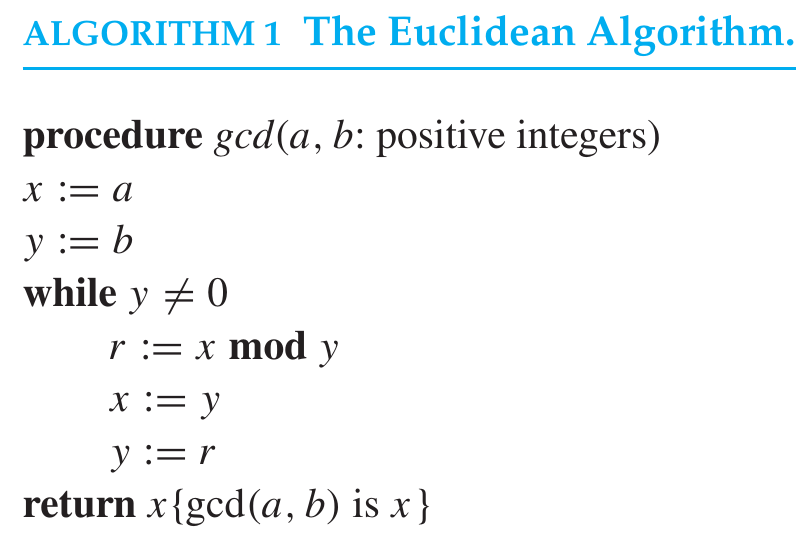
\includegraphics[width=0.5\textwidth]{euclids-algorithm}
    \end{center}

    Fjöldi deilinga sem reiknirit Evklíðs þarf til að reikna \emph{gcd(a,b)} þar sem $a \geq b$ er $O(\log b)$.
\end{frame}

\begin{frame}{Næst}
    Á föstudag: Forfallafyrirlestur Snorra Agnarssonar

    Á þriðjudag eftir viku: Dulkóðun (4.6), e.t.v. valið efni um leifareikning (4.4)
\end{frame}


\end{document}
